\documentclass[11pt]{article}
\usepackage[a4paper,margin=1in]{geometry}
\usepackage{amsmath,amssymb}
\usepackage[T1]{fontenc}
\usepackage{lmodern}
\usepackage{microtype}
\usepackage{graphicx}
\usepackage{xcolor}

\setlength{\parindent}{0pt}
\setlength{\parskip}{0.5em}

\newcommand{\promptbox}[1]{%
  \begingroup\setlength{\fboxsep}{10pt}\noindent
  \colorbox{blue!8}{\parbox{\dimexpr\linewidth-2\fboxsep\relax}{\textbf{Prompt. }#1}}
  \endgroup
}
\newcommand{\resultbox}[1]{%
  \begingroup\setlength{\fboxsep}{10pt}\noindent
  \colorbox{purple!8}{\parbox{\dimexpr\linewidth-2\fboxsep\relax}{\textbf{Result. }#1}}
  \endgroup
}
\newcommand{\examplebox}[1]{%
  \begingroup\setlength{\fboxsep}{10pt}\noindent
  \colorbox{green!8}{\parbox{\dimexpr\linewidth-2\fboxsep\relax}{\textbf{Example. }#1}}
  \endgroup
}

\title{\textbf{Book 1 --- Lecture 1 --- Interlude 1 --- Exercise 2}\\[2mm]
\large Vector Subtraction Rule}
\author{}
\date{}

\begin{document}
\maketitle

\promptbox{Work out the rule for vector subtraction.}

\section*{Rule}
Vector subtraction is defined componentwise:
\[
\mathbf{A}-\mathbf{B}=(A_1-B_1,\dots,A_n-B_n).
\]

Equivalent and often more useful form:
\[
\mathbf{A}-\mathbf{B}=\mathbf{A}+(-\mathbf{B}),
\]
where \(-\mathbf{B}\) is the additive inverse\footnote{The additive inverse of
\(\mathbf{B}\) is the vector that sums with \(\mathbf{B}\) to the zero vector.}
of \(\mathbf{B}\).

\section*{Geometric Interpretation}
\begin{itemize}
  \item If vectors share the same tail, \(\mathbf{A}-\mathbf{B}\) is the vector
  from the tip\footnote{The \emph{tip} is the arrowhead (terminal point) of a
  vector.} of \(\mathbf{B}\) to the tip of \(\mathbf{A}\).
  \item In 2D/3D drawings, this is equivalent to adding \(\mathbf{A}\) to the
  reversed arrow \(-\mathbf{B}\).
\end{itemize}

\section*{Quick Check in 2D}
\[
(3,-1)-(2,4)=(3-2,-1-4)=(1,-5).
\]

\resultbox{Vector subtraction is componentwise and equivalent to adding the
negative vector: \(\mathbf{A}-\mathbf{B}=\mathbf{A}+(-\mathbf{B})\).}

\examplebox{For \(\mathbf{A}=(3,-1)\) and \(\mathbf{B}=(2,4)\), one gets
\(\mathbf{A}-\mathbf{B}=(1,-5)\).}

\section*{Example Drawing}
The figure below visualizes \(\mathbf{A}=(3,-1)\), \(\mathbf{B}=(2,4)\), and
\(\mathbf{A}-\mathbf{B}=(1,-5)\). The dashed red arrow shows the
``tip of \(\mathbf{B}\) to tip of \(\mathbf{A}\)'' interpretation.

\begin{center}
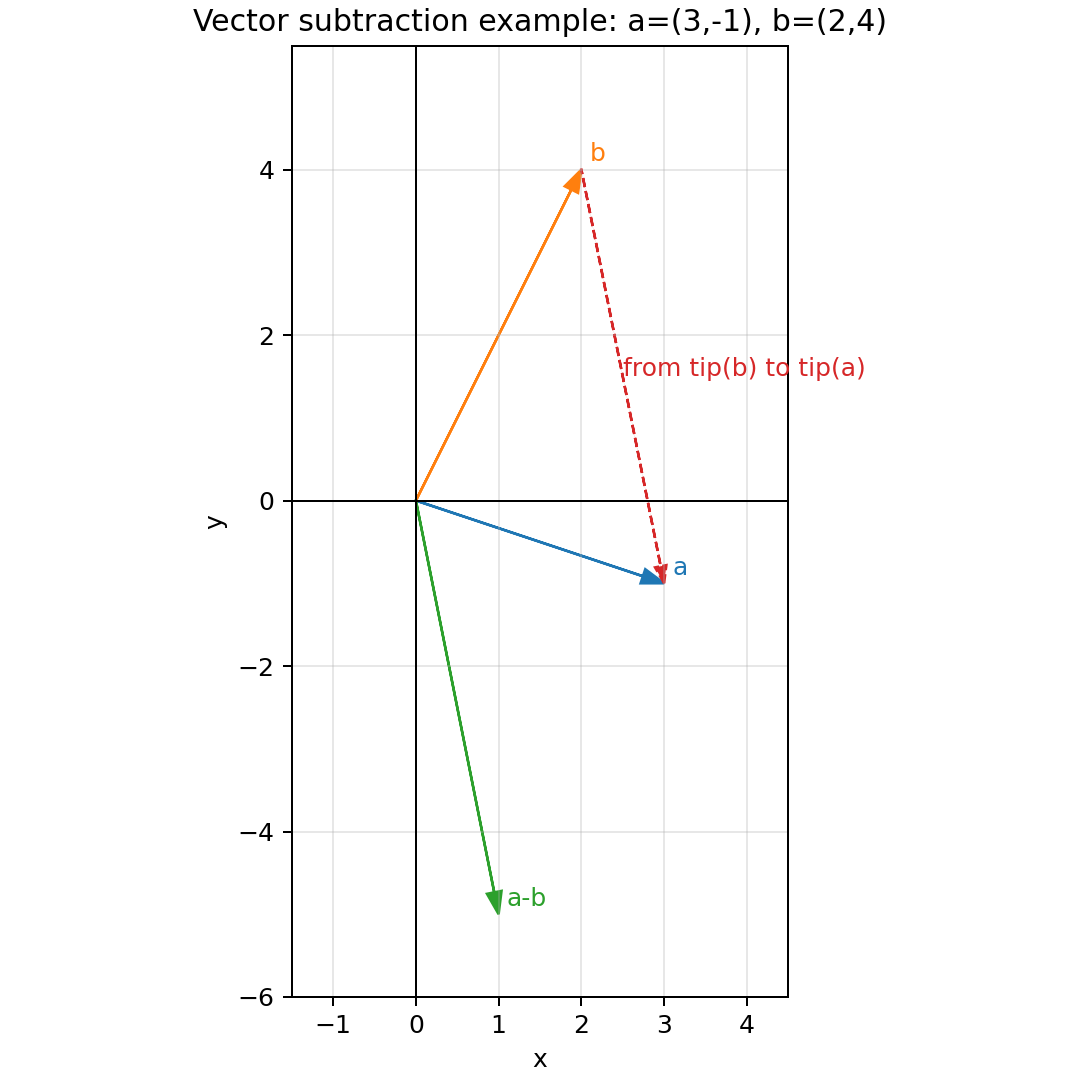
\includegraphics[width=0.72\textwidth]{exercise-02-vector-subtraction.png}
\end{center}

\end{document}
